% Format teze zasnovan je na paketu memoir
% http://tug.ctan.org/macros/latex/contrib/memoir/memman.pdf ili
% http://texdoc.net/texmf-dist/doc/latex/memoir/memman.pdf
% 
% Prilikom zadavanja klase memoir, navedenim opcijama se podešava 
% veličina slova (12pt) i jednostrano štampanje (oneside).
% Ove parametre možete menjati samo ako pravite nezvanične verzije
% mastera za privatnu upotrebu (na primer, u b5 varijanti ima smisla 
% smanjiti 
\documentclass[12pt,oneside]{memoir} 

% Paket koji definiše sve specifičnosti master rada Matematičkog fakulteta
\usepackage[latinica]{matfmaster} 
%
% Podrazumevano pismo je ćirilica.
%   Ako koristite pdflatex, a ne xetex, sav latinički tekst na srpskom jeziku
%   treba biti okružen sa \lat{...} ili \begin{latinica}...\end{latinica}.
%
% Opicija [latinica]:
%   ako želite da pišete latiniciom, dodajte opciju "latinica" tj.
%   prethodni paket uključite pomoću: \usepackage[latinica]{matfmaster}.
%   Ako koristite pdflatex, a ne xetex, sav ćirilički tekst treba biti
%   okružen sa \cir{...} ili \begin{cirilica}...\end{cirilica}.
%
% Opcija [biblatex]:
%   ako želite da koristite reference na više jezika i umesto paketa
%   bibtex da koristite BibLaTeX/Biber, dodajte opciju "biblatex" tj.
%   prethodni paket uključite pomoću: \usepackage[biblatex]{matfmaster}
%
% Opcija [b5paper]:
%   ako želite da napravite verziju teze u manjem (b5) formatu, navedite
%   opciju "b5paper", tj. prethodni paket uključite pomoću: 
%   \usepackage[b5paper]{matfmaster}. Tada ima smisla razmisliti o promeni
%   veličine slova (izmenom opcije 12pt na 11pt u \documentclass{memoir}).
%
% Naravno, opcije je moguće kombinovati.
% Npr. \usepackage[b5paper,biblatex]{matfmaster}

% Pomoćni paket koji generiše nasumičan tekst u kojem se javljaju sva slova
% azbuke (nema potrebe koristiti ovo u pravim disertacijama)
\usepackage[latinica]{pangrami}

% Datoteka sa literaturom u BibTex tj. BibLaTeX/Biber formatu
\bib{matfmaster-primer}

% Ime kandidata na srpskom jeziku (u odabranom pismu)
\autor{Katarina M. Dimitrijević}
% Naslov teze na srpskom jeziku (u odabranom pismu)
\naslov{Master iz matematike ili računarstva čiji je naslov jako dugačak}
% Godina u kojoj je teza predana komisiji
\godina{2015}
% Ime i afilijacija mentora (u odabranom pismu)
\mentor{dr Mika \textsc{Mikić}, redovan profesor\\ Univerzitet u Beogradu, Matematički fakultet}
% Ime i afilijacija prvog člana komisije (u odabranom pismu)
\komisijaA{dr Ana \textsc{Anić}, vanredni profesor\\ University of Disneyland, Nedođija}
% Ime i afilijacija drugog člana komisije (u odabranom pismu)
\komisijaB{dr Laza \textsc{Lazić}, docent\\ Univerzitet u Beogradu, Matematički fakultet}
% Ime i afilijacija trećeg člana komisije (opciono)
% \komisijaC{}
% Ime i afilijacija četvrtog člana komisije (opciono)
% \komisijaD{}
% Datum odbrane (odkomentarisati narednu liniju i upisati datum odbrane ako je poznat)
% \datumodbrane{}

% Apstrakt na srpskom jeziku (u odabranom pismu)
\apstr{%
\pangrami
}

% Ključne reči na srpskom jeziku (u odabranom pismu)
\kljucnereci{graf, algoritam, drvo, složenost}

\begin{document}
% ==============================================================================
% Uvodni deo teze
\frontmatter
% ==============================================================================
% Naslovna strana
\naslovna
% Strana sa podacima o mentoru i članovima komisije
\komisija
% Strana sa posvetom (u odabranom pismu)
\posveta{Mami, tati i dedi}
% Strana sa podacima o disertaciji na srpskom jeziku
\apstrakt
% Sadržaj teze
\tableofcontents*

% ==============================================================================
% Glavni deo teze
\mainmatter
% ==============================================================================

% ------------------------------------------------------------------------------
\chapter{Uvod}
% ------------------------------------------------------------------------------
\pangrami

\section{Minimalno povezujuće drvo}
Jedan od fundamentalnih grafovskih prolema je problem pronalaženja minimalnog povezujućeg (razapinjućeg) drveta. Ovaj problem podrazumeva pronalaženje povezanog podgrafa zadatog grafa koji sadrži sve čvorove polaznog grafa, a čija je ukupna cena minimalna. Primer jednog ovakvog drveta prikazan je na slici \ref{fig:MST}.

Ovaj problem ima primene u različitim domenima. Jedna od najčešćih primena ovog problema je u dizajnu raznih vrsta komunikacijskih mreža u slučaju kada je potrebno povezati sve čvorove mreže tako da između svaka dva čvora postoji jedinstven put, a da ukupna cena puta bude minimalna. Takođe, minimalno povezujuće drvo se koristi i za rešavanje problema klasterovanje, ali i za rešavanje nekih np-teških problema, npr. problema trgovačkog putnika.

U nastavku sledi nekoliko poglavlja u kojima je dat je pregled različitih algoritama za rešavanje ovog problema.

\begin{figure}[!ht]
  \centering
  \label{fig:MST}
  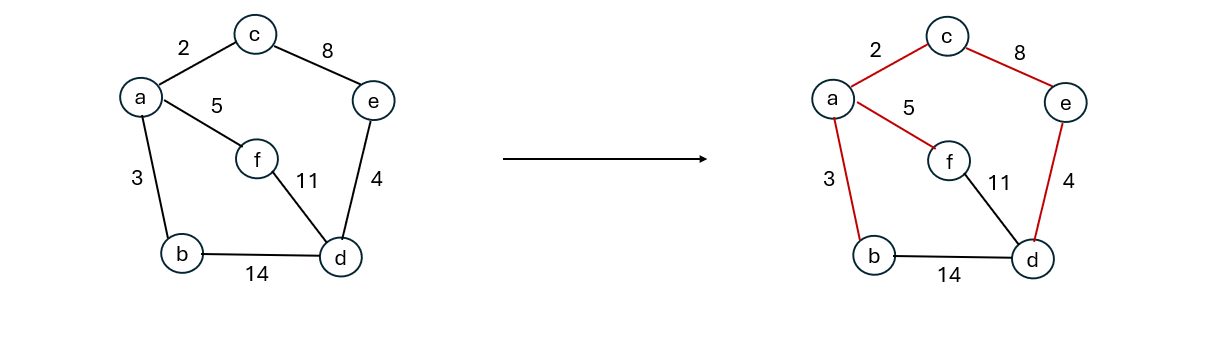
\includegraphics[width=1.0\textwidth]{matfmaster/MST.png}
  \caption{Primer minimalnog povezujućeg drveta}
\end{figure}



\section{Primov algoritam}
Prvi algoritam za konstruisanje minimalnog povezujućeg drveta koji će biti obrađen u ovom radu je Primov algoritam. Osmišljen je 1930. godine kao matematički algoritam u okviru teorije grafova, a 1957. godine je objavljen rad iz oblasti informatike u kome je, po drugi put, predstavljen isti algoritam.

Kako je minimalno povezujuće drvo zadato skupom grana, prirodno se nameće ideja da se ono može konstruisati dodavanjem jedne po jedne grane. Narenda grana se bira tako da bude najmanje težine od svih grana koje povezuju do tada konstruisano drvo sa čvorovima koji još uvek nisu dodati. Dokaz korektnosti ovako opisanog algoritma se može jednostavno sprovesti uz pomoć indukcije.

\textbf{Induktivna hipoteza}: Za povezan graf G, zadat skupom čvorova V i skupom grana E, u oznaci G=(V,E), može se konstruisati drvo T koje sadrži k grana, tako da je ono podgraf zadatog grafa.

\textbf{Baza indukcije}: Za bazu se uzima grana najmanje težine. Ako pretpostavimo da ona nije deo minimalnog povezujućeg drveta, njenim dodavanjem se zatvara neki ciklus. Uklanjanjem proizvoljne grane iz tog ciklusa dobija se drvo, ali sada manje ukupne cene, što je u kontradikciji sa time da se primenom ovog algoritma dobija drvo minimalne cene. Na osnovu navedenog se lako zaključuje da se grana minimalne težine mora naći u drvetu i zbog toga je pogodno uzeti je kao bazni slučaj.

\textbf{Induktivni korak}: Pretpostavlja se da je lako pronaći drvo T koje zadovoljava induktivnu hipotezu i koje se sastoji od k-1 grane. Postavlja se pitanje kako pronaći narednu granu. Ideja je slična kao i pri odabiru prve grane. Naime, posmatra se skup grana koje povezuju čvorove drveta T i čvorove koji se još uvek ne nalaze u T. Među njima se bira ona koja ima najmanju težinu, jer se u suprotnom može jednostavno doći do kontradikcije na isti način kao i pri odabiru prve grane.

Primov algoritam je zasnovan na istoj ideji kao i Dajkstrin algoritam za pronalaženje najkraćeg puta. Polazi se od praznog skupa grana i u svakoj iteraciji se dodaje po jedna grana čime se drvo proširuje. Do svakog čvora, iz skupa čvorova koji još uvek ne pripadaju drvetu T, pamti se cena putanje, a ukoliko ona ne postoji smatra se da iznoisi \( +\infty \). Nakon odabira naredne grane, proveravaju se cene grana do svih susednih čvorova i ukoliko je cena manja od cene putanje do tog čvora, koja je u prethodnim iteracijama izračunata, cena putanje se ažurira. Opisani postupak je skoro pa identičan Dajkstrinom algoritmu, izuzev što se kod Primovog algoritma putanje minimizuju po ukupnoj ceni putanje, a ne po broju grana. Stoga, složenost Primovog algoritma ekvivalentna je složenoisti Dajkstrinog i iznosi \( O((|E| + |V|) \log |V|) \). Smatra se prilično efikasnim algoritmom, naročito za retke grafove (one koji imaju malo grana).\\

\begin{figure}[!ht]
  \centering
  \label{fig:Prim}
  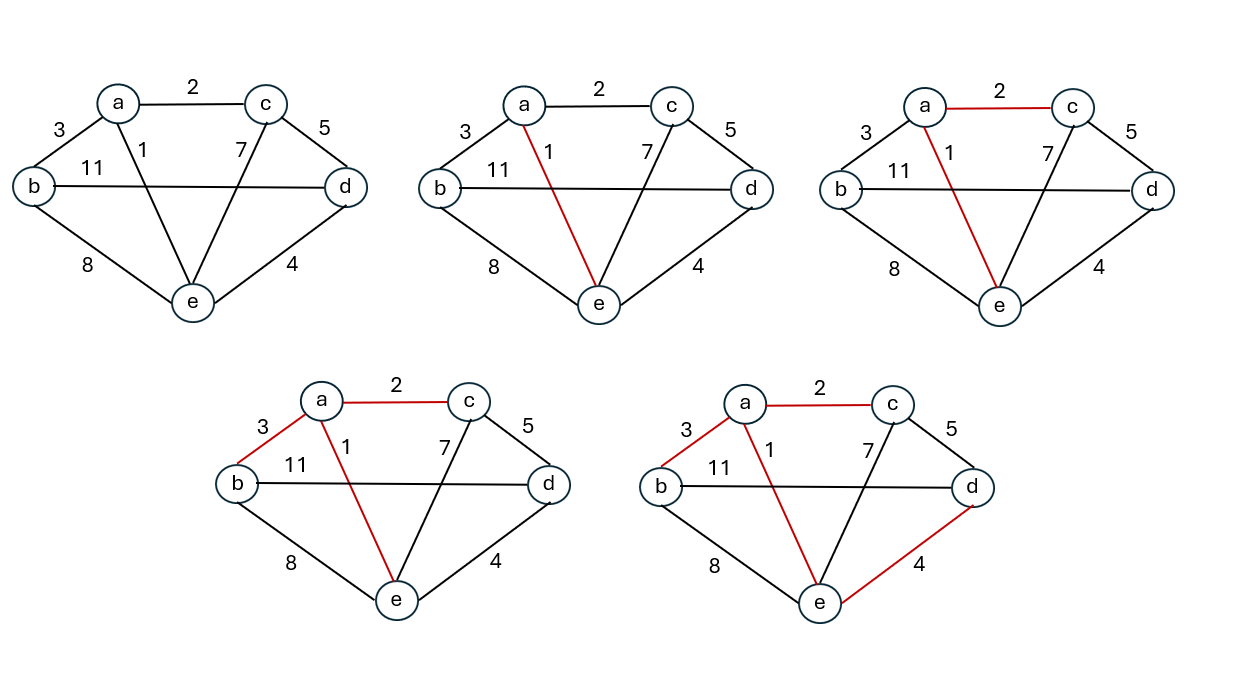
\includegraphics[width=1.0\textwidth]{matfmaster/PrimAlgo.png}
  \caption{Primer izvršavanja Primovog algoritma}
\end{figure}

Na slici \ref{fig:Prim} je ilustovan rad Primovog algoritma, korak po korak. Minimalno povezujuće stablo za zadati graf sa slike čine grane: \{a,e\}, \{a,c\}, \{a,b\} i \{e,d\}, a njegova ukupna cena iznosi 11. Kao što je i objašnjeno u prethodnom paragrafu, postupak čuvanja cena putanja do svih čvorova i njihovo ažuriranje kroz iteracije može se videti u tabeli \ref{tbl:Prim}. Prvi element i-te vrste tabele odgovara čvoru koji je dodat u i-toj iteraciji, dok ostali elementi te vrste odgovaraju cenama putanja između njega i ostalih koji još uvek ne pripadaju konstruisanom drvetu. Vrednost beskonačno označava da put između neka dva čvora još uvek nije poznat.\\

\begin{table}[h]
\centering
\label{tbl:Prim}
\begin{tabular}{|>{\centering}p{0.8cm}|>{\centering}p{0.8cm}|>{\centering}p{0.8cm}|>{\centering}p{0.8cm}|>{\centering}p{0.8cm}|>{\centering\arraybackslash}p{0.8cm}|}
\hline
 & a & b & c & d & e \\
\hline
a & - & a(3) & a(2) & \( \infty \) & a(1) \\
\hline
b & - & - & a(2) & b(11) & a(1) \\
\hline
c & - & - & - & e(4) & a(1) \\
\hline
d & - & - & - & - & a(1) \\
\hline
e & - & - & - & - & - \\
\hline
\end{tabular}
\caption{Cene putanja do čvorova kroz iteracije}
\end{table}

\section{Kruskalov algoritam}
Sledeći algoritam za konstrukciju minimalnog povezujućeg drveta koji će biti obrađen u ovom radu je Kruskalov algoritam. On je takođe, kao i Primov, primer \textit{pohlepnog algoritma} koji je nastao 1956. godine. Međutim, ideja na kojoj je ovaj algoritam zasnovan je nešto drugačija od prethodne, pa se i sama logika algoritma razlikuje od Primovog.

Naime, ideja je da se minimalno povezujuće stablo konstruiše dodavanjem jedne po jedne grane na trenutnu šumu, a ne na trenutno drvo kao što je to slučaj kod prethodnog. Sam algoritam započinje izvršavanje nad skupom čvorova, tako da svaki čvor predstavlja zasebno drvo. U svakoj iteraciji se uzima naredna grana, iz rastuće sortiranog skupa, na osnovu njihovih cena. Ukoliko čvorovi, koji su incidenti sa tekućom granom, pripadaju razlicitim stablima šume, ta grana se dodaje u tekuću šumu, dok se u suprotnom preskače. Dodavenjem grane se vrši spajanje stabala kojima pripadaju čvorovi trenutne grane. Na ovaj način se dodavanjem svake grane, broj stabala trenutne šume smanjuje za jedan. Lako se zaključuje da se postupak završava nakon dodavanja |V|-1 grane cime je formirano jedno drvo u kome postoji jedinstven put između svaka dva čvora, odnosno, koje ne sadrži cikluse. Trivijano se dokazuje da je opisanim postuponom zaista formirano povezujuće drvo. Takođe, intuitivno je jasno da je to drvo i minimalno, a to se može i pokazati.

Dokaz se jednostavno sprovodi svođenjem na kontradikciju. Naime, pretpostavimo da, iznad opisani, Kruskalov algoritam, vraća drvo K koje nije minimalno, dok je T minimalno povezujuće drvo. Kako nisu ista, ova dva drveta se moraju razlikovati na bar jednoj grani. Neka prva takva grana u rastući sortiranom nizu, bude ona koja povezuje čvorove a i b, u oznaci g(a, b). Kruskalov algoritam je konstruisan tako da iz sortiranog niza grana uzima svaku koja ne formira ciklus, tako da možemo da zaključimo na osnovu toga da grana g mora pripadati drvetu K, a ne pripada drvetu T. Po definiciji povezujućeg drveta, između čvorova a i b mora postojati jedinstven put. Na tom putu u T mora postojati bar jedna grana g1 koja je manje cene od grane g jer bi u suprotnom K moralo sadržati taj put (uzimajući jednu po jednu granu iz sortiranog niza), a on bi zajedno sa granom g formirao ciklus. Upravo izbacivanjem te grane g1 i dodavnjem grane g u drvo T, dobija se drvo manje ukupne cene, što je u kontradikciji sa polaznom pretpostavkom da je T minimalno.

\textbf{Analiza složenosti}: u implementaciji ovog algoritma se za spajanje dva drveta, prilikom dodavanja grane, kao i proveru da li grana pripada istom ili različitim drvetima, koristi veoma efikasna struktura, poznata kao union-find. Glavna petlja algoritma se izvršava |E| puta. U petlji se pozivaju operacije pronalaženje predstavnika (find) i uniranje stabala (union) složenosti \( O(\log |V|) \). Takođe, na samom početku je potrebno inicijalizovati union-find strukturu što je \( O(|V|) \), kao i izdvojiti i sortirati sve grane, što u proseku iznosi  \( O(|E|\log |E|) \). Sumiranjem svega navedenog i korišćenjem poznate nejednakosti $|E| \leq |V|^2$, dolazimo do ukupne složenosti \( O(|E|\log |V|) \). Slično kao i Primov, smatra se efikasnim algoritmom, ali naročito za retke grafove.

\begin{figure}[!ht]
  \centering
  \label{fig:Kruskal}
  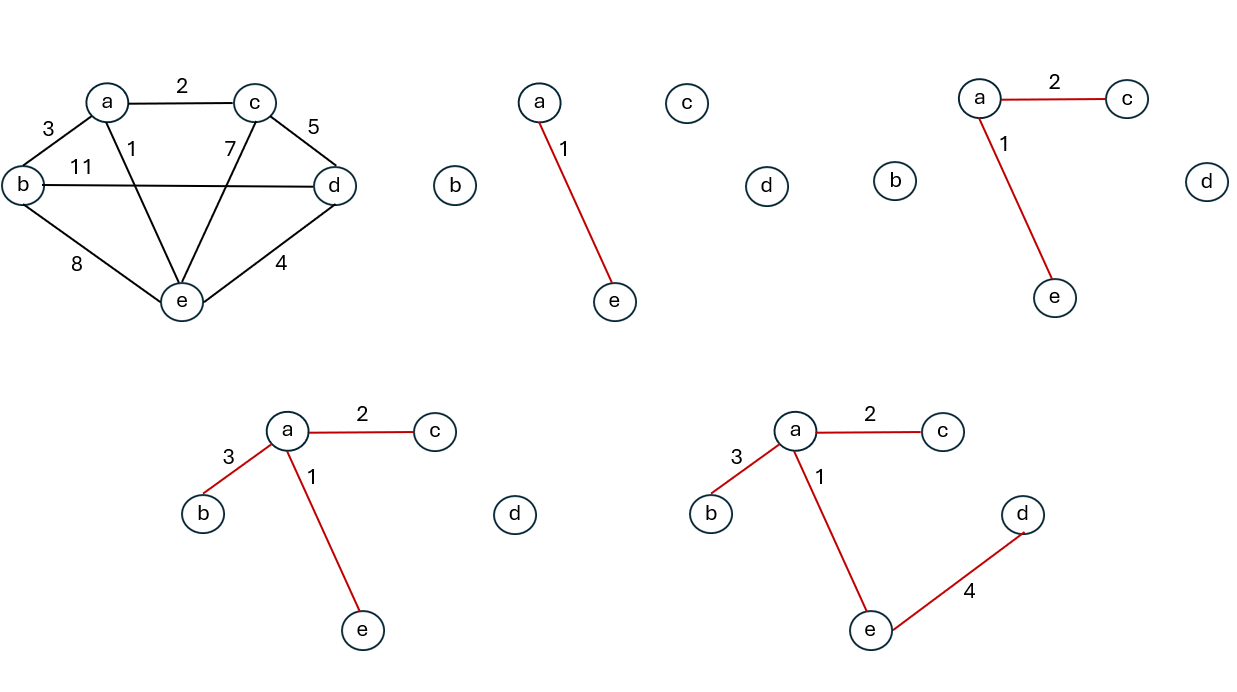
\includegraphics[width=1.0\textwidth]{matfmaster/KruskalAlgo.png}
  \caption{Primer izvršavanja Kruskalovog algoritma}
\end{figure}

Na slici \ref{fig:Kruskal} je prikazan primer izvršavanja Kruskalovog algoritma koji na ulazu dobija graf sa slike. Rad algoritma započinje nad skupom čvorova V, gde svaki od njih čini stalbo za sebe i zajedno formiraju tekuću šumu \{a\}, \{b\}, \{c\} i \{d\} i \{e\}. Uzima se jedna po jedna grana iz niza sortiranih grana i uključuje se samo ukoliko ne zatvara ciklus. Tekuću šumu nakon prve iteracije čine stabla: \{a, e\}, \{b\}, \{c\} i \{d\}, nakon druge: \{a, c, e\},  \{b\} i  \{d\} i  nakon treće \{a, b, c, e\} i \{d\}. Na samom kraju nastaje samo jedno stablo \{a, b, c, d, e\}, odnosno, algoritam se zaustavlja kada se konstruiše drvo koje sadrži |V|-1 granu.

\section{Boruvkin algoritam}
Boruvkin algoritam, nastao 1926. godine, je još jedan algoritam za pronalaženje minimalnog povezujućeg stabla zadatog grafa, koji takođe, kao i prethodna dva, spada u grupu \textit{pohlepnih algoritama}. Ideja na kojoj se zasniva je veoma intuitivna i jednostavna. Polazi se od skupa čvorova ulaznog grafa, gde se svaki od njih posmatra kao zasebna komponenta, odnosno, drvo, kao i kod Kruskalovog algoritma. Ideja je da se te komponente spajaju dok ne ostane samo jedna, koje je zapravo traženo minimalno povezujuće drvo početnog grafa i tada se algoritam zaustavlja. Na ovaj način se u svakom koraku dodaje po jedna grana na trenutnu šumu. Ono što se zapravo razlikuje u odnosu na spomenuti algoritam je način odabira grana, odnosno sama konstrukcije drveta.

U prvom koraku se za svaki čvor iz skupa V pronalazi grana najmanje cene koja je incidentna sa tim čvorom i ona se dodaje na trenutnu šumu. Ovime se broj komponenti smanjuje. Ovaj korak se ponavlja, s tim što se nakon prve iteracije više ne biraju grane koje povezuju pojedinačne čvorove, vec komponente. Postupak se zaustavlja kada ostane samo jedna komponenta. U svakom koraku se bira grana koja povezuje dve razlicite komponente, čime ne dolazi do zatvaranja ciklusa što je osnovni uslov za konstruisanje povezujućeg drveta grafa. Ovo se jednostavno može dokazati \textbf{indukcijom} po broju komponenti.

Za bazu indukcije se uzima slučaj gde je svaki čvor komponenta za sebe, tako da ima |V| komponenti. U nekom k-tom koraku se trenutna šuma sastoji od komponenti u kojima nema ciklusa jer su formirane dodavanjem jedne po jedne grane koje spajaju dve manje komponente, odnosno grana se dodaje samo ako joj krajevi pripadaju dvema razlicitim komponentama. Jasno je da će spajanjem komponenti na ovaj način, u jednom trenutku ostati jedna jedina komponenta koja sadrži sve čvorove, a ne sadrži cikluse, što je po definiciji povezujuće drvo. Sada jedino ostaje pokazati da je ovo drvo ujedno i minimalno, odnosno drvo najmanje ukupne cene.

\textbf{Dokaz} da je povezujuće drvo dobijeno opisanim postupkom minimalno se može sprovesti na isti način kao i slučaju Kruskalovog algoritma, metodom svođenja na kontradikciju.

U implementaciji ovog algoritma se novoformirana komponenta identifikuje svojim predstavnikom, a sve grane unutar jedne komponente se eliminišu. Takođe, prilikom spajanja komponenti granom najmanje cene, sve ostale grane između njih mogu biti eliminisane. Za potrebe ovih operacija se koristi efikasna, već ranije spomenuta, union-find struktura. 

\textbf{Analiza složenosti}: u svakoj iteraciji se na trenutnu šumu dodaje bar |V|/2 grana, čime se broj čvorova smanjuje bar dvostruko u odnosu na početni graf, a broj iteracija iznosi \( O(\log |V|) \). U svakoj od tih iteracija se svaka grana razmatra najviše jednom. Dakle, ukupna složenost iznosi \( O(|E|\log |V|) \). Iako ima istu složenost kao i Primov i Kruskalov algoritam, za razliku od njih, pokazuje se znatno efikasnijim na gustim grafovima. Takođe, njegova velika prednost je mogućnost paralelizacije.

\begin{figure}[!ht]
  \centering
  \label{fig:Boruvka}
  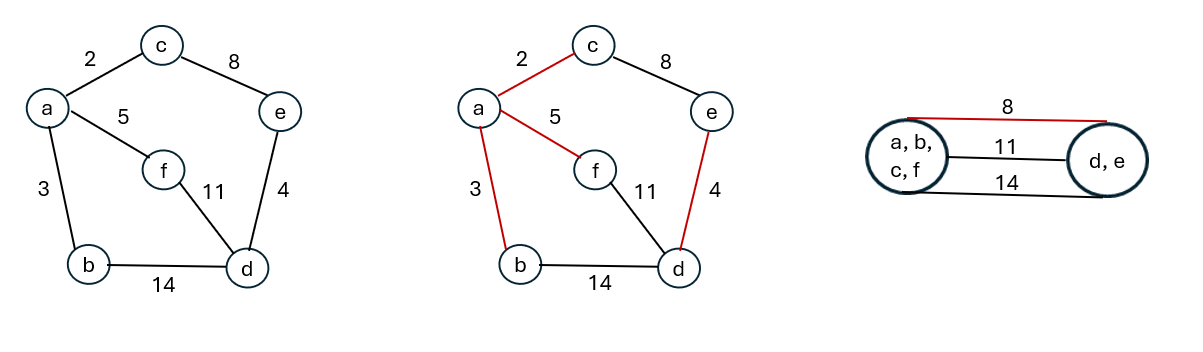
\includegraphics[width=1.0\textwidth]{matfmaster/BoruvkaAlgo.png}
  \caption{Primer izvršavanja Boruvka algoritma}
\end{figure}

Na slici \ref{fig:Boruvka} je prikazan primer izvršavanja Boruvkinog algoritma. U prvoj iteraciji se svaki čvor grafa iz skupa V=\{a, b, c, d, e, f\}\ posmatra kao zasebna komponenta. Za svaki od njih se pronalazi njemu incidentna grana najmanje cene tako da ga ona povezuje sa drugom komponentom. Pregled takvih grana za svaku od komponenti, nakon završene prve iteracije, dat je u tabeli \ref{tbl:boruvka1}.

\begin{table}
\centering
\label{tbl:boruvka1}
\begin{tabular}{|c|>{\centering}p{2cm}|c|}
\hline
 Komponenta & Grana & Cena\\ 
\hline
\{a\} & (a, c) & 2\\
\hline
\{b\} & (a, b) & 3\\
\hline
\{c\} & (a, c) & 2\\
\hline
\{d\} & (d, e) & 4\\
\hline
\{e\} & (d, e) & 4\\
\hline
\{f\} & (a, f) & 5\\
\hline
\end{tabular}
\caption{Grane obeležene u prvoj iteraciji}
\end{table}

Ove grane se označavaju i tako se formiraju nove komponente koje sadrže njima incidentne čvorove. Primenom operacija unije nastaju nove komponente i one sada postaju ulaz u drugu iteraciju algoritma. Postupak se ponavlja. Grane koje su obeležene u drugoj iteraciji su date u tabeli \ref{tbl:boruvka2}.

Obeležavanjem poslednje grane nastaje jedinstavena komponenta i algoritam se zaustavlja. Prolaskom kroz označene grane se konstruiše minimalno povezujuće drvo polaznog grafa. Njega čine grane: (a, c), (a, b), (a, f), (c, e) i (a, c), ukupne cene 22. 

\begin{table}
\centering
\label{tbl:boruvka2}
\begin{tabular}{|c|>{\centering}p{2cm}|c|}
\hline
 Komponenta & Grana & Cena\\ 
\hline
\{a, b, c, f\} & (c, e) & 8\\
\hline
\{d, e\} & (c, e) & 8\\
\hline
\end{tabular}
\caption{Grane obeležene u drugoj iteraciji}
\end{table}

\section{Reverse-delete algoritam}
Još jedan algoritam iz grupe \textit{pohlepnih algortama} za pronalaženje minimalnog povezujućeg drveta je delete-reverse algoritam. Algoritam na ulazu dobija neusmeren, težinski graf. Ideja je da se inicijalno grane sortiraju u opadajućem poretku, a zatim se razmatra, za svaku od njih, da li nakon njenog uklanjanja graf ostaje povezan. Ukoliko je to slučaj, trenutna grana se uklanja i nastavlja se dalje sa izvršavanjem. U protivnom se ta grana zadržava i prelazi se na sledeću iz sortiranog niza. Ova ideja je veoma jednostavna i podseća na već pominjanu ideju, bas onu na kojoj je zasnovan Kruskalov algoritam, s tim sto se kod njega grane, najpre sortirane u rastući poredak, razmatraju jedna po jedna i dodaju na trenutnu šumu, osim ukoliko formiraju ciklus. 

Iako se na osnovu samog opisa algoritma lako može zaključiti da on zaista daje minimalno povezujuće drvo, u nastavku sledi dokaz.
Prvi deo dokaza, odnosno tvrdnja da reverse-delete algoritam nalazi \textbf{drvo} je veoma jednostavano pokazati. Algoritam na ulazu dobija povezani, težinski graf G. Uklanjanjem jedne po jedne grane, uz uslov da graf sve vreme ostaje povezan, na kraju se ostaje graf koji sadrži inicijalni skup čvorova, ali iz koga su uklonjene sve grane koje formiraju neki ciklus, što je po definiciji drvo.
Drugi deo dokaza je malo komplikovaniji i odnosi se na \textbf{minimalnost} ovako dobijenog drveta. Ovo se može pokazati indukcijom. Naime, polazimo od povezanog grafa G i tvrdimo da u svakom trenutku njegov podgraf F, koji nastaje uklanjanjem grana iz G kroz iteracije, sadrži minimalno povezujuće drvo.

Ova tvrdnja je tačna pre prve iteracije algoritma, jer je inicijalno F=G, a kako je to povezan težinski graf, kao takav uvek sadrži minimalno povezujuće drvo T. Takođe, F može sadržati i neko drugo drvo, na primer drvo T'. U nekoj k-toj iteraciji, će biti izbačena grana e. Ukoliko ta grana ne pripada drvetu T, ono ostaje minimalno i T=T'. Međutim, ukoliko grana e pripada drvetu T, u tom slučaju njenim izbacivanjem znamo da graf G ostaje povezan, jer je to uslov koji algoritam sve vreme održava. Međutim, može se desiti da drvo T postane nepovezano. U tom slučaju mora postojati neki drugi put koji povezuje te dve komponente na koje je sada rastavljeno drvo T, što znači da je ranije je postojao ciklus u F. Jasno je da postoji neka grana e' iz tog ciklusa koja se nalazi van T, jer u suprotnom T ne bi bilo drvo. Tako da možemo da tvrdimo da ona pripada nekom drugom drvetu T' koje je takođe podgraf od F i da važi T'=T-e+e'. Lako je pokazati da je da je T' zaista drvo jer nastalo izbacivanjem grane e iz drveta T i dodavanjem nove grane e', tako da se na taj način zadržavaju svojstva drveta. Sada možemo takođe pokazati i da je drvo T' minimalno. Posmatrajmo weight(e) i weight(e'). Lako se pokazuje da nije moguće weight(e)>weight(e') jer je T minimalno povezujuće drvo. Takođe, nije moguće ni weight(e)<weight(e') jer algoritam uklanja grane u opadajućem redosledu što znači da bi onda grana e' bila razmatrana pre grane e i ovo dovodi do kontradikcije u razmatranom slučaju. Iz navedenog sledi da mora važiti da je weight(e)=weight(e'), odnosno da je T'=T, što znači da u svakoj iteraciji važi da F sadrži minimalno povezujuće drvo. Na samom kraju izvršavanja, sve grane koje učestvuju u nekom ciklusu su izbačene, što znači da je samo F drvo, odnosno, samo F je minimalno povezujuće drvo.

\textbf{Analiza složenosti}: vreme potrebno za sortiranje svih grana je \( O(|E|\log |E|) \). Nakon izbacivanja svake grane je neophodno pokrenuti neku pretragu kojom se proverava da li je graf ostao povezan (npr. DFS pretraga) čija složenost iznosi \( O(|E|+|V|) \). Dakle, ukupna vremenska složenost iznosi: \( O(|E|\log |E| + E(|E|+|V|))\).

\begin{figure}[!ht]
  \centering
  \label{fig:ReverseDelete}
  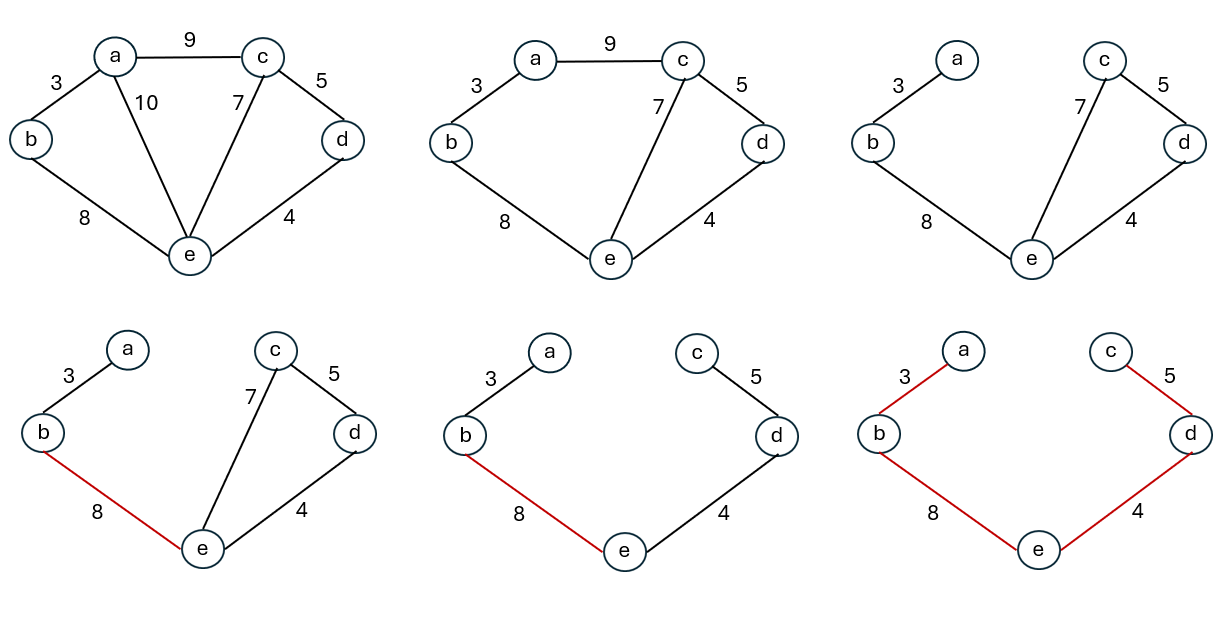
\includegraphics[width=1.0\textwidth]{matfmaster/ReverseDeleteAlgo.png}
  \caption{Primer izvršavanja reverse-delete algoritma}
\end{figure}

Na slici \ref{fig:ReverseDelete} je prikazano izvršavanje algoritma. Grane se razmatraju jedna po jedna iz opadajući sortiranog niza i uklanjaju se sve koje ulaze u sastav nekog ciklusa. Na primeru su najpre uklonjene grane (a,e) i (a,c). Sledeća koja je dosla na red za uklanjanje je grana (b,e), međutim, njenim brisanjem bi graf postao nepovezan tako da se ona preskače. Zatim, uklanja se i (c,e). Sledeća je (b,e), ali ona se ne sme ukoniti, kao nijedna od preostalih grana jer nijedna od njih ne ulazi u sastav nekog ciklusa. Drugim rečima, grane koje su preostale čine minimalno povezujuće drvo. 


...

\end{document}
